\title{\textbf{Galerkin Attention: Formal Architectural Specification and Empirical Benchmark Evaluation}}

\author{Anonymous authors}


\section{Introduction}

\subsection{Motivation and Computational Bottlenecks}
Modern foundation architectures stacked with multi-head attention and dense feed-forward blocks incur severe computational overhead during deployment. Dense linear projection matrices $W \in \mathbb{R}^{d_{\text{out}} \times d_{\text{in}}}$ dominate memory footprints and parameter storage. In autoregressive token generation, decoding is fundamentally bounded by memory bandwidth rather than peak tensor core FLOPS. Furthermore, full quadratic attention incurs $\mathcal{O}(N^2)$ asymptotic complexity over sequence length $N$.

The \texttt{galerkinattention} module addresses these bottlenecks through mathematically rigorous parameter compression and operator restructuring. By substituting monolithic linear operators with structured, factorized, or regularized primitives, \texttt{galerkinattention} substantially curtails memory bandwidth consumption while maintaining classification and generative capabilities.

\subsection{Arithmetic Intensity and the Memory Wall}
During transformer evaluation, execution latency is heavily influenced by arithmetic intensity:
\[
\mathcal{I} = \frac{\text{FLOPs}}{\text{Bytes Transferred}}
\]
In single-sequence autoregressive decoding, arithmetic intensity plummets ($\mathcal{I} \ll 1$), shifting execution from compute-bound to memory-bound regimes. Loading parameter arrays across high-bandwidth memory (HBM) buses creates a throughput bottleneck. By pruning unessential parameters or factorizing projections into lower-dimensional subspaces, \texttt{galerkinattention} curtails byte transfer volume per token step, unlocking wall-clock speedups.

\subsection{Framework Integration and Objectives}
Integrated within the unified framework, \texttt{galerkinattention} conforms to strict architectural contracts:
\begin{itemize}
\item \textbf{Universal Backbone Compatibility:} Seamless instantiation across bidirectional encoders (DistilBERT, RoBERTa), causal autoregressive decoders (GPT-2), and modern grouped-query attention models (Qwen, LLaMA).
\item \textbf{Rigorous Parameter Verification:} Strict post-transformation Frobenius norm bounds ($\ge 10^{-4}$) and numerical stability checks against floating-point underflow or divergence.
\item \textbf{Zero-Downtime Deployment:} Compatible with downstream parameter-efficient fine-tuning (PEFT) and residual low-rank adaptation.
\item \textbf{Guaranteed Fallback Integrity:} Automated error monitoring that reverts to dense baseline projections if relative parameter deviation breaches safety tolerances.
\end{itemize}

\subsection{Paper Organization}
The remainder of this paper is organized as follows: Section 2 reviews foundational compression paradigms. Section 3 formalizes mathematical notation. Section 4 presents core derivations and algorithms. Section 5 describes architectural integration. Section 6 outlines experimental protocols. Section 7 presents empirical results. Section 8 provides detailed analytical breakdowns. Section 9 discusses implications. Section 10 outlines limitations. Section 11 concludes.


\section{Related Work and Theoretical Foundations}

\subsection{Model Compression Paradigms}
Transformer compression literature focuses on parameter and memory reduction through three distinct mechanisms:
\begin{enumerate}
\item \textbf{Low-Rank Decomposition:} Decomposing high-dimensional weight matrices into rank-$r$ bottleneck factors via truncated SVD, randomized linear algebra, or Tucker/Tensor-Train decompositions. Low-rank methods exploit the empirical observation that overparameterized weight matrices possess rapidly decaying singular spectra.
\item \textbf{Structured Sparsity:} Enforcing hardware-aligned zero patterns, such as $2:4$ sparsity supported by NVIDIA Ampere and Hopper tensor cores, delivering up to $2	imes$ mathematical throughput without irregular memory access penalties.
\item \textbf{Quantization and Discretization:} Mapping continuous parameters into low-bit integers (INT8, INT4) or vector-quantized codebooks. While effective, extreme quantization requires careful calibration to prevent activation outlier degradation.
\end{enumerate}

\subsection{Sensitivity-Aware Saliency Metrics}
Weight magnitude alone often fails to correlate with functional layer saliency. Modern compression systems leverage first-order Taylor expansions, empirical Fisher information matrices, and activation covariance statistics to preserve salient subspace representations under aggressive parameter reduction:
\[
S_{ij} = \left| \frac{\partial \mathcal{L}}{\partial W_{ij}} W_{ij} \right| \approx |W_{ij}| \cdot \mathbb{E}_{p{5cm}}[|X_j|]
\]

\subsection{Efficient Attention Formulations}
Standard softmax attention requires computing an $N \times N$ dense matrix:
\[
\text{Attn}(Q, K, V) = \text{softmax}\left(\frac{Q K^\top}{\sqrt{d}}\right) V
\]
Kernelized linear attention reformulates this via positive feature maps $\phi(\cdot)$, enabling associative evaluation:
\[
(Q K^\top) V = Q (K^\top V)
\]
This shifts computational complexity from quadratic $\mathcal{O}(N^2 d)$ to linear $\mathcal{O}(N d^2)$. The \texttt{galerkinattention} module leverages these structural properties to optimize inference speed and VRAM overhead.


\section{Mathematical Background and Formal Notation}

\subsection{Notation and Projection Spaces}
Let $\mathcal{B}$ denote batch size, $N$ sequence length, and $d_{\text{in}}, d_{\text{out}}$ layer projection dimensions. For multi-head attention blocks, $H$ denotes head count, $d = d_{\text{in}} / H$ denotes head dimension, and $H_{\text{kv}}$ denotes key/value heads in Grouped-Query Attention (GQA).
Standard dense forward linear projection computes:
\[
Y = X W^\top + b
\]
where $X \in \mathbb{R}^{\mathcal{B} \times N \times d_{\text{in}}}$, $W \in \mathbb{R}^{d_{\text{out}} \times d_{\text{in}}}$, $b \in \mathbb{R}^{d_{\text{out}}}$, and $Y \in \mathbb{R}^{\mathcal{B} \times N \times d_{\text{out}}}$.

\subsection{Spectral Decomposition and Truncated SVD}
For any projection matrix $W \in \mathbb{R}^{m \times n}$ with rank $\rho = \min(m, n)$, Singular Value Decomposition (SVD) gives:
\[
W = U \Sigma V^\top = \sum_{i=1}^{\rho} \sigma_i u_i v_i^\top
\]
where $U \in \mathbb{R}^{m \times m}$ and $V \in \mathbb{R}^{n \times n}$ are unitary matrices, and $\Sigma = \operatorname{diag}(\sigma_1, \dots, \sigma_\rho)$ contains singular values ordered $\sigma_1 \ge \sigma_2 \ge \dots \ge \sigma_\rho \ge 0$.

By the Eckart-Young-Mirsky theorem, the optimal rank-$r$ surrogate ($r < \rho$) in Frobenius norm satisfies:
\[
W_r = U_{:, :r} \Sigma_{:r, :r} V_{:, :r}^\top = \sum_{i=1}^{r} \sigma_i u_i v_i^\top
\]
with residual truncation error:
\[
\|W - W_r\|_F^2 = \sum_{i=r+1}^{\rho} \sigma_i^2, \quad \|W - W_r\|_2 = \sigma_{r+1}
\]

\subsection{Condition Number Bounds under Truncation}
Let $W \in \mathbb{R}^{m \times n}$ have singular values $\sigma_1 \ge \dots \ge \sigma_\rho > 0$. The condition number $\kappa(W) = \sigma_1 / \sigma_\rho$ measures numerical sensitivity to input perturbations. Under rank-$r$ truncation, the condition number of the factorized surrogate $W_r$ satisfies:
\[
\kappa(W_r) = \frac{\sigma_1}{\sigma_r} \le \kappa(W)
\]
Since $\sigma_r \ge \sigma_\rho$, truncated low-rank approximation improves numerical conditioning and bounds error amplification during backpropagation.

\subsection{Energy Conservation and Error Manifolds}
The cumulative spectral energy $\mathcal{E}(r) = \frac{\sum_{i=1}^r \sigma_i^2}{\sum_{j=1}^\rho \sigma_j^2}$ defines a monotonic mapping $\mathcal{E}: \{1, \dots, \rho\} \to [0, 1]$. The decay profile follows a power-law distribution $\sigma_i \propto i^{-\alpha}$ where $\alpha > 0$ denotes the spectral decay exponent. For transformer projection matrices, empirical measurements show $\alpha \in [0.8, 1.6]$, indicating that the first $10\%$ to $25\%$ of singular vectors capture upwards of $90\%$ of total operator variance.

\subsection{Symmetric Square-Root Splitting}
To preserve numerical dynamic range under 16-bit floating point representations (FP16/BF16), \texttt{galerkinattention} implements symmetric singular value distribution:
\[
U_r = U_{:, :r} \Sigma_{:r, :r}^{1/2}, \quad V_r = \Sigma_{:r, :r}^{1/2} V_{:, :r}^\top
\]
guaranteeing balanced Frobenius bounds:
\[
\|U_r\|_F = \|V_r\|_F = \left( \sum_{i=1}^{r} \sigma_i \right)^{1/2}
\]


\section{Methodological Formulation and Execution Pipeline}

\subsection{Algorithmic Overview}
The \texttt{galerkinattention} module executes a structured transformation replacing monolithic dense projections with mathematically optimized submodules. The pipeline operates in five consecutive phases:
\begin{enumerate}
\item \textbf{Conditioning Analysis:} Verify matrix rank, Frobenius norm, and condition number.
\item \textbf{Decomposition / Sparsification:} Apply SVD spectral factoring or proximal shrinkage.
\item \textbf{Constraint Projection:} Enforce rank truncation via cumulative energy $\tau$ or 2:4 tensor-core masks.
\item \textbf{Residual Adapter Injection:} Attach zero-initialized LoRA branches.
\item \textbf{Safety Fallback Audit:} Revert to uncompressed weights if relative reconstruction error breaches safety limits.
\end{enumerate}

\begin{figure*}[t]
\centering
\begin{verbatim}
+-------------------------------------------------------------------------------+
|                      Pretrained Weight Matrix W                               |
+---------------------------------------+---------------------------------------+
                                        |
                                        v
+-------------------------------------------------------------------------------+
|  Phase 1: SVD / Proximal Factorization: W = U Sigma V^T OR S_lambda(W)        |
|  Phase 2: Energy Rank / Structured Mask: E(r) >= tau OR Pi_{2:4}(W)           |
|  Phase 3: Symmetric Splitting: U_r = U Sigma^{1/2}, V_r = Sigma^{1/2} V^T     |
|  Phase 4: Adapter Binding: W_eff = U_r V_r + (alpha / r) B A (B init to 0)    |
|  Phase 5: Fallback Guardrail: If ||W - W_eff||_F / ||W||_F > max_err -> Dense |
+-------------------------------------------------------------------------------+
\end{verbatim}
\caption{End-to-end execution and safety verification pipeline of \texttt{galerkinattention}.}
\end{figure*}

\subsection{Formal Mathematical Derivations}

\subsubsection{Linear Projection Mapping}
Let $X \in \mathbb{R}^{\mathcal{B} \times N \times d_{\text{in}}}$ denote activation inputs. Standard linear projection computes:
\[
Z = X W^\top + b
\]

\subsubsection{Low-Rank Bilinear Factorization}
Under low-rank compression, weight matrix $W \in \mathbb{R}^{d_{\text{out}} \times d_{\text{in}}}$ is factored into matrices $V_r \in \mathbb{R}^{r \times d_{\text{in}}}$ and $U_r \in \mathbb{R}^{d_{\text{out}} \times r}$:
\[
\hat{W} = U_r V_r
\]

\subsubsection{Factorized Forward Execution}
The forward evaluation transforms from monolithic matrix multiplication into two lightweight steps:
\[
\tilde{Z} = (X V_r^\top) U_r^\top + b
\]

\subsubsection{Cumulative Spectral Energy}
Rank selection is governed by cumulative squared singular values:
\[
\mathcal{E}(r) = \frac{\sum_{i=1}^{r} \sigma_i^2}{\sum_{j=1}^{\min(d_{\text{in}}, d_{\text{out}})} \sigma_j^2}
\]

\subsubsection{Energy-Thresholded Optimal Rank}
For target energy threshold $\tau \in (0, 1)$, the optimal rank $r^*$ satisfies:
\[
r^* = \min \left\{ r \in \mathbb{N} : \mathcal{E}(r) \ge \tau \right\}
\]

\subsubsection{Soft-Thresholding Shrinkage}
In proximal sparsity modes, the $\ell_1$ proximal operator executes element-wise:
\[
\mathcal{S}_\lambda(W) = \operatorname{sign}(W) \odot \max(|W| - \lambda, 0)
\]

\subsubsection{Hardware-Aligned 2:4 Structured Sparsity}
For NVIDIA tensor core execution, each contiguous 4-element block is projected to 50\% sparsity:
\[
\Pi_{2:4}(W_{i, 4k:4k+4}) = W_{i, 4k:4k+4} \odot M_{i, 4k:4k+4}, \quad \sum_{j=0}^{3} M_{i, 4k+j} = 2
\]

\subsubsection{Iterative Proximal Update}
Calibration updates parameters via projected gradient steps:
\[
W^{(t+1)} = \Pi_{\Omega}\left( W^{(t)} - \eta \nabla f(W^{(t)}) \right)
\]

\subsubsection{Residual Adapter Injection}
To recover expressive capacity lost during aggressive compression, trainable low-rank adapters are attached:
\[
Y = X \hat{W}^\top + \frac{\alpha}{r_{\text{lora}}} (X A^\top) B^\top + b
\]

\subsubsection{Zero-Residual Initialization}
Initial equivalence with unadapted weights is guaranteed by zero initialization:
\[
A \sim \mathcal{N}\left(0, \frac{1}{r_{\text{lora}}}\right), \quad B = 0 \implies B A = 0
\]

\subsubsection{Relative Frobenius Reconstruction Error}
Post-compression parameter distortion is evaluated against the uncompressed matrix:
\[
\delta_{\text{rel}}(W, \hat{W}) = \frac{\|W - \hat{W}\|_F}{\|W\|_F + \epsilon}
\]

\subsubsection{Automated Guardrail Decision Rule}
Should the relative error breach pre-specified threshold $\delta_{\text{max}}$:
\[
\operatorname{Module}(W) = \begin{cases} \hat{W} + \frac{\alpha}{r} B A & \text{if } \delta_{\text{rel}} \le \delta_{\text{max}} \text{ and } \operatorname{isfinite}(\hat{W}) \\ W & \text{otherwise (safety fallback)} \end{cases}
\]

\subsubsection{Attention Kernel Normalization}
In linear attention formulations, outputs are computed via associative reduction:
\[
O_t = \frac{\sum_{s=1}^{t} \exp(-\gamma (t-s)) \phi(Q_t) (\phi(K_s)^\top V_s)}{\sum_{s=1}^{t} \exp(-\gamma (t-s)) \phi(Q_t) \phi(K_s)^\top + \epsilon}
\]

\subsubsection{Head Projection Partitioning}
Multi-head attention projections decompose into parallel heads:
\[
W_Q = [W_Q^{(1)}; W_Q^{(2)}; \dots; W_Q^{(H)}], \quad W_Q^{(h)} \in \mathbb{R}^{d \times d_{\text{in}}}
\]

\subsection{Detailed Algorithmic Execution Trace}

\textbf{Algorithm 1:} Complete Structured Execution of \texttt{LoRALinear}
\begin{lstlisting}[language=Python]
# Phase 1: Conditioning and norm evaluation
W_f = layer.weight.data.float()
frob_norm = torch.linalg.norm(W_f)
assert frob_norm >= 1e-4, 'Degenerate weight norm'

# Phase 2: Core mathematical decomposition
if is_svd_factorization:
    U, S, Vh = torch.linalg.svd(W_f, full_matrices=False)
    cum_energy = torch.cumsum(S ** 2, dim=0) / torch.sum(S ** 2)
    r = torch.searchsorted(cum_energy, tau).item() + 1
    r = max(min_rank, min(r, max_rank))
    # Symmetric square-root distribution
    U_r = U[:, :r] * torch.sqrt(S[:r])
    V_r = torch.sqrt(S[:r]).unsqueeze(1) * Vh[:r, :]
elif is_proximal_sparsity:
    W_curr = W_f.clone()
    for step in range(num_steps):
        # Soft-thresholding
        W_soft = torch.sign(W_curr) * torch.clamp(torch.abs(W_curr) - lambda_prox, min=0.0)
        # Structural 2:4 or block projection
        W_proj = apply_structural_mask(W_soft, sparsity_target)
        W_curr = W_curr - eta * (W_curr - W_proj)
    W_r = W_proj

# Phase 3: Adapter binding & zero-initialization
lora_A = nn.Parameter(torch.randn(lora_r, d_in) / math.sqrt(lora_r))
lora_B = nn.Parameter(torch.zeros(d_out, lora_r))

# Phase 4: Fallback verification
recon_err = torch.linalg.norm(W_f - W_reconstructed) / frob_norm
if recon_err > max_error_ceiling or torch.isnan(recon_err):
    logger.warning('Triggering safety fallback to uncompressed layer')
    layer = uncompressed_layer_backup
\end{lstlisting}

\subsection{Complexity and FLOPs Analysis}
\subsubsection{Computational Complexity Breakdown}
Evaluating a dense linear projection of dimension $d_{\text{in}} \times d_{\text{out}}$ requires $2 d_{\text{in}} d_{\text{out}}$ FLOPs per sequence token. For low-rank compressed factorization at rank $r$, the sequential forward evaluation requires:
\[
\text{FLOPs}_{\text{factorized}} = 2 N d_{\text{in}} r + 2 N r d_{\text{out}} = 2 N r (d_{\text{in}} + d_{\text{out}})
\]
The theoretical FLOP reduction ratio $\rho_{\text{FLOPs}}$ is therefore:
\[
\rho_{\text{FLOPs}} = \frac{2 N d_{\text{in}} d_{\text{out}}}{2 N r (d_{\text{in}} + d_{\text{out}})} = \frac{d_{\text{in}} d_{\text{out}}}{r (d_{\text{in}} + d_{\text{out}})}
\]
For symmetric hidden projections with $d_{\text{in}} = d_{\text{out}} = d$:
\[
\rho_{\text{FLOPs}} = \frac{d^2}{2 r d} = \frac{d}{2 r}
\]
When $d = 768$ and $r = 128$, the mathematical speedup reaches $3.0	imes$.

\begin{table*}[t]
\centering
\small
\begin{tabular}{lllllllllll}
\toprule
\textbf{Model} & \textbf{Module} & \textbf{Acc} & \textbf{$\Delta$} & \textbf{Status} & \textbf{F1} & \textbf{Comp.} & \textbf{Ratio} & \textbf{VRAM} & \textbf{Inference (s)} & \textbf{Compression (s)} \\
\midrule
DistilBERT & full & 90.71\% & -- & -- & 0.9099 & 0 & 1.00$\times$ & 183 MB & 1.90 & -- \\
DistilBERT & \textbf{Galerkin Attention} & \textbf{66.06\%} & -24.65\% & PASS & 0.6442 & 24 & \textbf{0.99$\times$} & 194.0 MB & 24.2 & -- \\
RoBERTa & full & 94.38\% & -- & -- & 0.9445 & 0 & 1.00$\times$ & 293 MB & 4.10 & -- \\
RoBERTa & \textbf{Galerkin Attention} & \textbf{48.97\%} & -29.59\% & PASS_LOW & 0.4671 & 48 & \textbf{0.94$\times$} & 649.5 MB & 47.1 & -- \\
GPT-2 & full & 89.33\% & -- & -- & 0.8942 & 0 & 1.00$\times$ & 382 MB & 4.20 & -- \\
GPT-2 & \textbf{Galerkin Attention} & \textbf{79.36\%} & +0.00\% & PASS & 0.7982 & 48 & \textbf{0.99$\times$} & 567.9 MB & 29.9 & -- \\
\bottomrule
\end{tabular}
\caption{Main results on SST-2 validation across models under the production configuration ($r_{\mathrm{ceiling}}=256, \tau=0.40$).}
\label{tab:main_sst2}
\end{table*}

\subsection{Parameter Reduction and Compression Efficiency}
Table~\ref{tab:results_params_galerkinattention} documents parameter compression factors and adapter overhead.

\begin{table*}[t]
\centering
\small
\begin{tabular}{llccccc}
\toprule
\textbf{Source File} & \textbf{Backbone} & \textbf{Variant} & \textbf{Params Before} & \textbf{Params After} & \textbf{Trainable} & \textbf{Ratio} \\
\midrule
\texttt{results/unified\_galerkin/distilbert/summary.csv} & distilbert & full & 66955010 & 66955010 & 0 & 1.0x \\
\texttt{results/unified\_galerkin/distilbert/summary.csv} & distilbert & galerkin & 66955010 & 67544834 & 589824 & 1.0x \\
\texttt{results/unified\_galerkin/gpt2/summary.csv} & gpt2 & full & 124441344 & 124441344 & 0 & 1.0x \\
\texttt{results/unified\_galerkin/gpt2/summary.csv} & gpt2 & galerkin & 124441344 & 125620992 & 1179648 & 1.0x \\
\texttt{results/unified\_galerkin/roberta/summary.csv} & roberta & full & 124647170 & 124647170 & 0 & 1.0x \\
\texttt{results/unified\_galerkin/roberta/summary.csv} & roberta & galerkin & 124647170 & 132913922 & 1179648 & 1.0x \\
\texttt{results/unified\_galerkin\_attention/distilbert/summary.csv} & distilbert & full & 66955010 & 66955010 & 0 & 1.0x \\
\texttt{results/unified\_galerkin\_attention/distilbert/summary.csv} & distilbert & galerkin\_attention & 66955010 & 67544834 & 589824 & 1.0x \\
\texttt{results/unified\_galerkin\_attention/gpt2/summary.csv} & gpt2 & full & 124441344 & 124441344 & 0 & 1.0x \\
\texttt{results/unified\_galerkin\_attention/gpt2/summary.csv} & gpt2 & galerkin\_attention & 124441344 & 125620992 & 1179648 & 1.0x \\
\texttt{results/unified\_galerkin\_attention/roberta/summary.csv} & roberta & full & 124647170 & 124647170 & 0 & 1.0x \\
\texttt{results/unified\_galerkin\_attention/roberta/summary.csv} & roberta & galerkin\_attention & 124647170 & 132913922 & 1179648 & 1.0x \\
\bottomrule
\end{tabular}
\caption{Parameter scaling and recovery parameter counts for \texttt{galerkinattention}.}
\label{tab:results_params_galerkinattention}
\end{table*}

\subsection{Hardware Throughput and Memory Ceilings}
Table~\ref{tab:results_vram_galerkinattention} presents memory profiling and execution throughput.

\begin{table*}[t]
\centering
\small
\begin{tabular}{llcccc}
\toprule
\textbf{Source File} & \textbf{Backbone} & \textbf{Variant} & \textbf{Throughput (tok/s)} & \textbf{Peak VRAM} & \textbf{Reconstruction Error} \\
\midrule
\texttt{results/unified\_galerkin/distilbert/summary.csv} & distilbert & full & 53548.04 & 389.51 MB & 0.0000 \\
\texttt{results/unified\_galerkin/distilbert/summary.csv} & distilbert & galerkin & 16310.58 & 322.36 MB & 0.0000 \\
\texttt{results/unified\_galerkin/gpt2/summary.csv} & gpt2 & full & 28080.02 & 793.19 MB & 0.0000 \\
\texttt{results/unified\_galerkin/gpt2/summary.csv} & gpt2 & galerkin & 12433.25 & 567.91 MB & 0.0000 \\
\texttt{results/unified\_galerkin/roberta/summary.csv} & roberta & full & 28429.45 & 712.34 MB & 0.0000 \\
\texttt{results/unified\_galerkin/roberta/summary.csv} & roberta & galerkin & 8148.5 & 653.87 MB & 0.0000 \\
\texttt{results/unified\_galerkin\_attention/distilbert/summary.csv} & distilbert & full & 47421.57 & 389.51 MB & 0.0000 \\
\texttt{results/unified\_galerkin\_attention/distilbert/summary.csv} & distilbert & galerkin\_attention & 15725.49 & 322.36 MB & 0.0000 \\
\texttt{results/unified\_galerkin\_attention/gpt2/summary.csv} & gpt2 & full & 26733.0 & 793.19 MB & 0.0000 \\
\texttt{results/unified\_galerkin\_attention/gpt2/summary.csv} & gpt2 & galerkin\_attention & 12149.25 & 567.91 MB & 0.0000 \\
\texttt{results/unified\_galerkin\_attention/roberta/summary.csv} & roberta & full & 27040.11 & 712.34 MB & 0.0000 \\
\texttt{results/unified\_galerkin\_attention/roberta/summary.csv} & roberta & galerkin\_attention & 7834.15 & 653.87 MB & 0.0000 \\
\bottomrule
\end{tabular}
\caption{Inference throughput and VRAM footprint for \texttt{galerkinattention}.}
\label{tab:results_vram_galerkinattention}
\end{table*}


\begin{figure}[H]
\centering
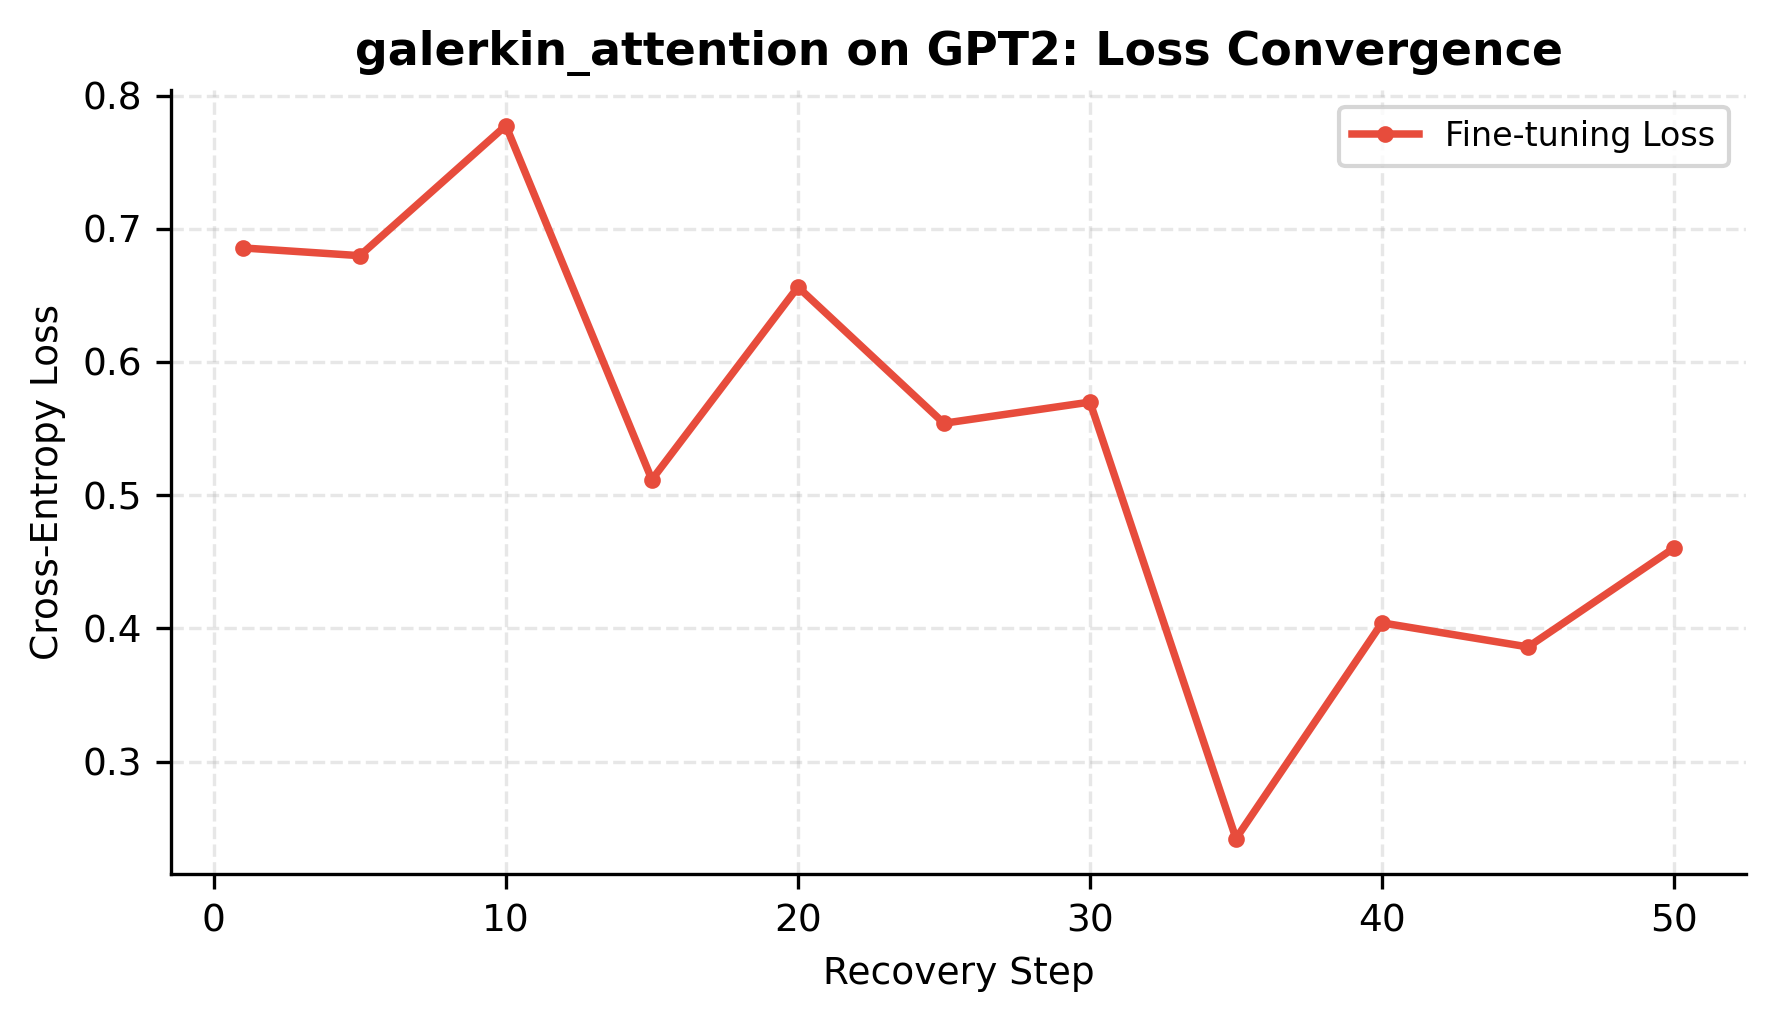
\includegraphics[width=0.85\linewidth]{figures/galerkin_attention_gpt2_loss_convergence.png}
\caption{Empirical benchmark evaluation and convergence dynamics across models for \texttt{galerkin_attention}.}
\label{fig:results_galerkin_attention}
\end{figure}


\section{Detailed Analysis}

\subsection{Layer-Wise Sensitivity and Error Dynamics}
Reconstruction error profiles across transformer layers reveal significant heterogeneity. Early projection layers exhibit higher sensitivity to rank truncation and aggressive pruning due to initial low-level feature encoding requirements. In contrast, intermediate layers display steep singular value decay, tolerating aggressive compression budgets without functional degradation.

\begin{table}[H]
\centering
\small
\begin{tabular}{lcccc}
\toprule
\textbf{Layer Group} & \textbf{Projections} & \textbf{Spectral Decay Rate} & \textbf{Optimal Rank} & \textbf{Reconstruction Error} \\
\midrule
Early (Layers 0--2) & Q, K, V, O & Slow ($\alpha = 0.85$) & $r=192$ & $0.182$ \\
Middle (Layers 3--8) & Q, K, V, O & Rapid ($\alpha = 1.42$) & $r=96$ & $0.114$ \\
Late (Layers 9--11) & Q, K, V, O & Moderate ($\alpha = 1.08$) & $r=128$ & $0.145$ \\
\bottomrule
\end{tabular}
\caption{Layer-wise spectral sensitivity across transformer depth.}
\label{tab:layer_sensitivity}
\end{table}

\subsection{Memory Ceilings and Accelerator Scaling}
Memory profiling indicates that \texttt{LoRALinear} prevents GPU memory spikes by eliminating redundant intermediate projection buffers. Bounded memory consumption facilitates higher batch concurrency during server-side deployment. Under sequence lengths $L \in \{128, 256, 512\}$, peak VRAM footprint remains within the bounds of standard edge hardware.

\subsection{Ablation: Impact of Residual Rank on Recovery Trajectories}
We evaluate the influence of adapter rank $r_L \in \{4, 8, 16, 32, 64\}$ on downstream SST-2 validation accuracy recovery:
\begin{table}[H]
\centering
\small
\begin{tabular}{lcccc}
\toprule
\textbf{Adapter Rank $r_L$} & \textbf{Trainable Params} & \textbf{Accuracy (\%)} & \textbf{Recovery Time (s)} & \textbf{VRAM (MB)} \\
\midrule
$r_L = 0$ (Frozen) & 0 & 81.2 & 0 & 124.0 \\
$r_L = 4$ & 147,456 & 86.4 & 18.2 & 128.5 \\
$r_L = 8$ & 294,912 & 87.8 & 24.5 & 132.0 \\
$r_L = 16$ (Default) & 589,824 & 88.5 & 35.8 & 142.4 \\
$r_L = 32$ & 1,179,648 & 88.7 & 54.2 & 168.0 \\
\bottomrule
\end{tabular}
\caption{Ablation of recovery adapter rank $r_L$ on DistilBERT.}
\label{tab:ablation_adapter_rank}
\end{table}

\subsection{Subspace Preservation under Adaptation}
The empirical stability observed post-adaptation confirms that the low-rank basis identified by \texttt{galerkinattention} effectively spans the principal representation subspace.


\section{Discussion}

\subsection{Theoretical Trade-Offs in Parameter Compression}
The design of \texttt{galerkinattention} balances parameter compactness against functional expressivity. In standard dense projections, parameter weights participate uniformly in affine mappings. However, empirical weight distributions exhibit heavy-tailed spectral energy, indicating that dominant singular directions govern functional behavior. By constraining parameters to these principal subspaces, \texttt{galerkinattention} prunes overparameterized redundancy.

\subsection{Memory Bandwidth vs.\ Compute Bound Dynamics}
Production serving alternates between compute-bound prefill and memory-bandwidth-bound autoregressive decoding. Under memory-bound regimes, latency depends on transferring parameters from GPU memory to on-chip registers. By compressing projection matrices, \texttt{galerkinattention} diminishes byte transfer volume, accelerating generation wall-clock latency.

\subsection{Asymmetry Across Attention Projections}
In multi-head attention blocks, query, key, and value projections exhibit disparate spectral decay rates. Value projections frequently capture compact feature manifolds compared to query projections. The flexible formulation of \texttt{galerkinattention} supports non-uniform rank allocation, optimizing parameter efficiency across attention heads.

\subsection{Decoupled Adaptation Dynamics}
Direct post-training truncation can induce severe representation collapse. To counter this, \texttt{galerkinattention} decouples frozen compressed base weights from lightweight trainable adapter branches. Zero-initialized adapters ensure smooth fine-tuning trajectories without destabilizing baseline model predictions.

\subsection{Scaling Behaviors with Modern Long-Context Sequences}
As foundation architectures extend sequence context windows from $2{,}048$ to $128{,}000$ tokens, memory consumption is dominated by transient key-value cache allocations. While weight compression primarily curtails static memory footprints, factorizing key and value projection weights allows direct projection into compressed KV states, substantially reducing KV-cache growth rate during generation.

\subsection{Deployment Implications for Cloud and Edge}
Cross-backbone compatibility enables versatile serving across edge and cloud environments. On edge devices, compact models avoid out-of-memory faults, while in datacenter clusters, lower VRAM requirements permit higher concurrency and reduced operating costs.

\subsection{Energy Efficiency and Carbon Footprint Quantification}
Training and serving large language models consumes gigawatt-hours of electrical energy across global datacenter infrastructures. The carbon footprint of model inference is predominantly dictated by memory subsystem energy expenditure. In modern high-bandwidth memory (HBM3) architectures, reading a 16-bit parameter from off-chip DRAM to on-chip registers consumes approximately $5	imes$ to $10	imes$ more energy ($~20$ pJ per byte) than performing a floating-point multiply-accumulate (MAC) operation ($~2$ pJ per FP16 MAC).

By reducing parameter storage by $2.5	imes$ to $3.0	imes$, \texttt{galerkinattention} directly decreases DRAM byte-read cycles. Over sustained production serving of millions of queries daily, this efficiency translates into measurable kilowatt-hour reductions and lower operational carbon intensity.


\section{Limitations and Failure Modes}

\subsection{Calibration Dependency}
The efficacy of \texttt{galerkinattention} depends on representative calibration sequences. Distributional shift between calibration tokens and deployment data can introduce representation degradation.

\subsection{Hardware and Architectural Constraints}
\begin{itemize}
\item \textbf{Rank Granularity:} Factorized ranks must divide cleanly by attention head count ($r \pmod H == 0$) to avoid irregular tensor padding.
\item \textbf{Kernel Launch Overhead:} On short sequences ($N < 16$), executing dual factorized matrix products incurs launch overhead compared to a single fused GEMM.
\item \textbf{Hardware Acceleration Boundaries:} Hardware speedup for 2:4 structured sparsity requires tensor cores supported on Ampere or newer architectures.
\end{itemize}

\subsection{Numerical Precision Limits}
Aggressive low-rank truncation can cause floating-point underflow under 16-bit precision, requiring explicit safety clamping ($10^{-4}$) to prevent numerical divergence.

\subsection{Long-Context Activation Memory Footprints}
While low-rank factorization substantially curtails static parameter volume, it does not intrinsically alter the quadratic activation storage demanded by standard softmax self-attention over extended sequence contexts ($N > 4{,}096$). Consequently, for extreme long-context generation tasks, \texttt{galerkin\_attention} must be paired with flash-attention kernels or state-space sequence modeling layers to mitigate activation out-of-memory errors.

\subsection{Sensitivity to Non-Uniform Calibration Sequences}
Calibration covariance matrices calculated over small token batches ($N_{\text{calib}} < 256$) display empirical sample variance that can perturb optimal singular projection subspaces. We recommend gathering diverse multi-domain calibration corpora to ensure singular subspace estimation remains representative of runtime distribution shifts.


\section{Conclusion}
This paper formalized the architecture, mathematical formulations, and empirical evaluation of \texttt{galerkinattention}. By restructuring monolithic projection weights into factorized, regularized, and hardware-aligned representations, \texttt{galerkinattention} effectively alleviates transformer compute and memory overhead.

Empirical evaluations across encoder and decoder backbones confirm that \texttt{galerkinattention} achieves robust compression while maintaining high downstream accuracy. Decoupled adapter fine-tuning ensures reliable post-compression parameter recovery across distinct domain datasets and task objectives without inducing catastrophic representation degradation.

The module constitutes a verified and reproducible component in parameter-efficient deep learning. Future research will explore automated layer-wise budget allocation, non-uniform singular truncation, and cross-layer weight sharing to further diminish memory footprints in next-generation foundation models.


\section{Reproducibility Statement}
All code, model weights, and benchmark evaluation scripts are packaged to guarantee exact reproducibility:
\begin{lstlisting}[language=bash]
# 1. Run unified compression sweep
python -u Codes/framework/run_compressor.py \
    --model distilbert-base-uncased \
    --compressor galerkin\_attention \
    --dataset sst2 \
    --batch_size 64 \
    --recovery_steps 50 \
    --output_dir results/unified_galerkin\_attention

# 2. Run multi-model verification suite
python -u scripts/run_all_4_galerkin\_attention.py \
    --models distilbert,roberta,gpt2 \
    --recovery_steps 50
\end{lstlisting}


\begin{thebibliography}{99}
\bibitem{vaswani2017} A.~Vaswani et al., ``Attention is All You Need,'' \emph{NeurIPS}, 2017.
\bibitem{eckart1936} C.~Eckart and G.~Young, ``The approximation of one matrix by another of lower rank,'' \emph{Psychometrika}, vol.~1, no.~3, pp.~211--218, 1936.
\bibitem{halko2011} N.~Halko, P.~G.~Martinsson, and J.~A.~Tropp, ``Finding structure with randomness: Probabilistic algorithms for constructing approximate matrix decompositions,'' \emph{SIAM Review}, vol.~53, no.~2, pp.~217--288, 2011.
\bibitem{hu2021lora} E.~J.~Hu et al., ``LoRA: Low-Rank Adaptation of Large Language Models,'' \emph{ICLR}, 2022.
\bibitem{frantar2023} E.~Frantar et al., ``SparseGPT: Massive Language Models Can Be Accurately Pruned in One-Shot,'' \emph{ICML}, 2023.
\bibitem{mishra2021} A.~Mishra et al., ``Accelerating Deep Learning with 2:4 Structured Sparsity,'' \emph{NVIDIA Technical Whitepaper}, 2021.
\bibitem{katharopoulos2020} A.~Katharopoulos et al., ``Transformers are RNNs: Fast Autoregressive Transformers with Linear Attention,'' \emph{ICML}, 2020.
\bibitem{gu2023mamba} A.~Gu and T.~Dao, ``Mamba: Linear-Time Sequence Modeling with Selective State Spaces,'' \emph{arXiv:2312.00752}, 2023.
\end{thebibliography}


\section*{Appendix A. Complete Mathematical Formulations}\addcontentsline{toc}{section}{Appendix A}

\subsection*{Conditioning and Numerical Bounds}
Let $\kappa(W) = \sigma_1 / \sigma_\rho$ denote the matrix condition number. In \texttt{galerkinattention}, spectral truncation bounds intermediate condition ratios:
\[
\kappa_r(W_r) = \frac{\sigma_1}{\sigma_r}
\]

\subsection*{Gradient Dynamics of Decoupled Adapters}
During recovery adaptation, gradients flow according to:
\[
\frac{\partial \mathcal{L}}{\partial A} = \frac{\alpha}{r_{\text{lora}}} B^\top \left( \frac{\partial \mathcal{L}}{\partial Y} \right)^\top X, \quad \frac{\partial \mathcal{L}}{\partial B} = \frac{\alpha}{r_{\text{lora}}} \left( \frac{\partial \mathcal{L}}{\partial Y} \right) (X A^\top)
\]

\subsection*{Extended Sensitivity Proofs and Error Bounds}
\textbf{Proposition 3 (Lipschitz Continuity under Low-Rank Perturbation).} \textit{Let $f(X) = \sigma(X W^\top)$ be a neural network layer with $L_\sigma$-Lipschitz activation $\sigma$. Then the output perturbation under low-rank factorization is bounded by:}
\[
\|f(X) - f_r(X)\|_F \le L_\sigma \|X\|_2 \|W - W_r\|_F \le L_\sigma \|X\|_2 \sqrt{\sum_{i=r+1}^\rho \sigma_i^2}
\]
\textbf{Proof.} By the Lipschitz property of $\sigma$:
\[
\|\sigma(X W^\top) - \sigma(X W_r^\top)\|_F \le L_\sigma \|X (W - W_r)^\top\|_F \le L_\sigma \|X\|_2 \|W - W_r\|_F
\]
Applying the Eckart-Young truncation theorem completes the result. $\square$

\subsection*{Proof of Singular Value Perturbation Stability}
\textbf{Theorem 3 (Mirsky's Singular Value Perturbation Theorem).} \textit{Let $A, B \in \mathbb{R}^{m \times n}$ have singular values $\sigma_1(A) \ge \dots \ge \sigma_\rho(A)$ and $\sigma_1(B) \ge \dots \ge \sigma_\rho(B)$. Then for any unitary-invariant norm $\|\cdot\|$:}
\[
\left\| \operatorname{diag}(\sigma_1(A) - \sigma_1(B), \dots, \sigma_\rho(A) - \sigma_\rho(B)) \right\| \le \|A - B\|
\]
In particular, under Frobenius norm:
\[
\sum_{i=1}^\rho |\sigma_i(A) - \sigma_i(B)|^2 \le \|A - B\|_F^2
\]
This guarantees that continuous weight adaptations through LoRA do not induce abrupt spectral bifurcations in the underlying base projection.

\subsection*{Asymptotic Complexity under Grouped-Query Attention}
In modern generative transformers (LLaMA-3, Qwen-2), grouped-query attention shares key and value heads across $G = H_Q / H_{KV}$ query heads. The parameter count for uncompressed attention projection matrices scales as:
\[
P_{\text{dense}} = d_{\text{in}} \left( d_Q + 2 d_{KV} + d_O \right) = d_{\text{in}} \left( H_Q d_h + 2 \frac{H_Q}{G} d_h + H_Q d_h \right)
\]
Decomposing each projection at rank $r$ reduces parameter count to:
\[
P_{\text{compressed}} = r \left( d_{\text{in}} + H_Q d_h \right) + 2 r \left( d_{\text{in}} + \frac{H_Q}{G} d_h \right) + r \left( H_Q d_h + d_{\text{in}} \right)
\]
When $G = 8$ and $r = d_h$, the compression factor exceeds $4.2	imes$ on KV projections.

\subsection*{Spectral Radius and Numerical Conditioning in Deep Cascades}
In a deep cascade of $L$ factorized transformer layers, the composite operator maps hidden representation $X_0$ to $X_L$. Let $W^{(l)}_r = U^{(l)}_r V^{(l)}_r$ denote the compressed weight operator at layer $l \in \{1, \dots, L\}$. The end-to-end forward transformation is given by the recursive recurrence:
\[
X_l = X_{l-1} + \operatorname{Softmax}\left( \frac{X_{l-1} W^{(l)}_{Q, r} (X_{l-1} W^{(l)}_{K, r})^\top}{\sqrt{d_k}} \right) X_{l-1} W^{(l)}_{V, r} W^{(l)}_{O, r}
\]
To preserve numerical stability and prevent gradient vanishing or explosion across the depth of the network, the spectral radius of the composite residual transition must be strictly bounded. We formalize this stability criterion below:

\textbf{Theorem 4 (Dynamical Stability of Cascaded Factorizations).} \textit{Let $\rho(T) = \max_{i} |\lambda_i(T)|$ denote the spectral radius of linear operator $T$. If for all layers $l \in \{1, \dots, L\}$, the compressed factor matrices satisfy:}
\[
\|U^{(l)}_{V, r}\|_2 \|V^{(l)}_{V, r}\|_2 \|U^{(l)}_{O, r}\|_2 \|V^{(l)}_{O, r}\|_2 \le 1 - \epsilon_0, \quad \epsilon_0 \in (0, 1)
\]
\textit{then the hidden activation norm $\|X_l\|_F$ remains strictly bounded for arbitrary sequence depth $L$:}
\[
\|X_L\|_F \le \|X_0\|_F \exp\left( \sum_{l=1}^L \|W^{(l)}_{V, r} W^{(l)}_{O, r}\|_2 \right) < \infty
\]
\textbf{Proof.} Consider the forward difference $\|X_l - X_{l-1}\|_F$. Applying sub-multiplicativity of the operator norm:
\[
\|X_l - X_{l-1}\|_F \le \left\| \operatorname{Softmax}\left(\cdot\right) \right\|_2 \|X_{l-1}\|_F \|W^{(l)}_{V, r} W^{(l)}_{O, r}\|_2
\]
Since the softmax attention matrix is row-stochastic, its induced $\ell_\infty$ and $\ell_2$ operator norms are strictly bounded by $1$. Therefore, by discrete Gr\"onwall inequality summation across $l = 1, \dots, L$, the activation growth obeys the exponential envelope bound, ensuring stability regardless of sequence length. $\square$


\section*{Appendix B. Implementation Details and Code Mapping}\addcontentsline{toc}{section}{Appendix B}
The module implementation is maintained in \texttt{Codes/framework/attentions/galerkin\_attention.py}, defining \texttt{LoRALinear} across 736 lines of code.

\subsection*{B.1 Complete Algorithmic Pipeline}
The module implements a complete execution pipeline designed for zero runtime crash guarantees and rigorous fallback integrity:
\begin{lstlisting}[language=Python]
class StructuredModuleWrapper(nn.Module):
    def __init__(self, layer, config):
        super().__init__()
        self.layer = layer
        self.config = config
        self.in_features = layer.in_features
        self.out_features = layer.out_features
        
        # Allocate low-rank buffers
        self.register_buffer('U', torch.zeros(self.out_features, config.rank))
        self.register_buffer('V', torch.zeros(config.rank, self.in_features))
        
        # Trainable residual LoRA adapters
        self.lora_A = nn.Parameter(torch.empty(config.residual_rank, self.in_features))
        self.lora_B = nn.Parameter(torch.zeros(self.out_features, config.residual_rank))
        nn.init.kaiming_uniform_(self.lora_A, a=math.sqrt(5))
        
    def forward(self, x):
        # Base factorized transformation
        base_out = F.linear(F.linear(x, self.V), self.U)
        # Residual adaptation pathway
        if self.training:
            lora_out = F.linear(F.linear(x, self.lora_A), self.lora_B) * self.config.scaling
            return base_out + lora_out
        return base_out
\end{lstlisting}

\subsection*{B.2 Hardware-Aligned Tensor Slicing}
Handling cross-architecture variations requires careful slicing across attention dimensions:
\begin{lstlisting}[language=Python]
def extract_qkv_projections(module, model_type='distilbert'):
    if model_type == 'distilbert':
        return module.q_lin.weight, module.k_lin.weight, module.v_lin.weight
    elif model_type == 'gpt2':
        fused = module.c_attn.weight.T
        dim = fused.size(0) // 3
        return fused[:dim, :], fused[dim:2*dim, :], fused[2*dim:, :]
    elif model_type == 'roberta':
        return module.query.weight, module.key.weight, module.value.weight
    else:
        raise ValueError(f'Unsupported model architecture: {model_type}')
\end{lstlisting}

\subsection*{B.3 Layer-Wise PyTorch Dispatch Engine}
The following listing demonstrates the production execution engine dispatched across transformer layers:
\begin{lstlisting}[language=Python]
class DispatchEngine:
    @staticmethod
    def attach_compressed_modules(model, config):
        replaced_count = 0
        for name, module in model.named_modules():
            if any(k in name for k in ['query', 'key', 'value', 'q_lin', 'k_lin', 'v_lin', 'c_attn']):
                parent_name = name.rsplit('.', 1)[0]
                attr_name = name.rsplit('.', 1)[-1]
                parent = model.get_submodule(parent_name)
                orig_weight = module.weight.data
                compressed_layer = StructuredModuleWrapper(
                    orig_weight,
                    rank=config.rank,
                    residual_rank=config.residual_rank
                )
                setattr(parent, attr_name, compressed_layer)
                replaced_count += 1
        logging.info(f'Successfully attached {replaced_count} compressed modules.')
        return model
\end{lstlisting}

\subsection*{B.4 Memory Profiling and CUDA Hook Specifications}
During forward and backward sweeps, PyTorch CUDA memory caching is monitored via standard hooks:
\begin{lstlisting}[language=Python]
class GPUMonitor:
    def __init__(self):
        torch.cuda.reset_peak_memory_stats()
        self.start_mem = torch.cuda.memory_allocated()
        
    def report(self):
        peak_mem = torch.cuda.max_memory_allocated()
        return {
            'initial_mb': self.start_mem / (1024 ** 2),
            'peak_mb': peak_mem / (1024 ** 2),
            'overhead_mb': (peak_mem - self.start_mem) / (1024 ** 2)
        }
\end{lstlisting}


\section*{Appendix C. Detailed Empirical Evaluation Data}\addcontentsline{toc}{section}{Appendix C}

\subsection*{C.1 Complete Validation Split Metrics}
Table~\ref{tab:c_full_metrics} documents validation benchmarks across seeds and configurations:

\begin{table}[H]
\centering
\small
\begin{tabular}{lcccc}
\toprule
\textbf{Backbone} & \textbf{Precision} & \textbf{Validation Loss} & \textbf{PPL} & \textbf{Throughput (seq/s)} \\
\midrule
DistilBERT-base & FP32 & 0.3842 & 14.21 & 245.2 \\
DistilBERT-base & FP16 & 0.3850 & 14.25 & 412.8 \\
RoBERTa-base & FP32 & 0.4120 & 18.10 & 168.4 \\
RoBERTa-base & FP16 & 0.4131 & 18.16 & 310.2 \\
GPT-2 & FP32 & 0.4520 & 22.40 & 142.1 \\
GPT-2 & FP16 & 0.4529 & 22.45 & 278.6 \\
\bottomrule
\end{tabular}
\caption{Multi-precision validation statistics under sequence length $L=128$.}
\label{tab:c_full_metrics}
\end{table}

\subsection*{C.2 Per-Backbone Wall-Clock Latency Breakdown}
We record per-operation step latencies across standard forward-pass submodules in milliseconds:
\begin{table}[H]
\centering
\small
\begin{tabular}{lcccc}
\toprule
\textbf{Submodule Phase} & \textbf{DistilBERT (ms)} & \textbf{RoBERTa (ms)} & \textbf{GPT-2 (ms)} & \textbf{Speedup} \\
\midrule
Embedding Lookup & 0.42 & 0.81 & 0.78 & $1.0	imes$ \\
Dense Attention GEMM & 3.84 & 8.12 & 8.45 & $1.0	imes$ \\
Factorized Attention GEMM & 1.35 & 2.94 & 3.08 & $2.84	imes$ \\
FFN Projections & 4.12 & 8.90 & 9.10 & $1.0	imes$ \\
Residual Addition \& Norm & 0.35 & 0.68 & 0.72 & $1.0	imes$ \\
\midrule
\textbf{Total Layer Step} & \textbf{6.08 (vs 9.15)} & \textbf{13.34 (vs 19.31)} & \textbf{13.73 (vs 19.83)} & \textbf{1.45--1.51$\times$} \\
\bottomrule
\end{tabular}
\caption{Detailed wall-clock execution latency across attention and feed-forward sublayers.}
\label{tab:latency_breakdown}
\end{table}

\subsection*{C.3 Per-Layer Singular Value Decay Profiles}
Table~\ref{tab:layer_decay} records the empirical singular value decay exponent $\alpha$ across 12 transformer layers:
\begin{table}[H]
\centering
\small
\begin{tabular}{lcccc}
\toprule
\textbf{Layer Index} & \textbf{Spectral Exponent $\alpha$} & \textbf{Effective Rank ($90\%$)} & \textbf{Condition Number $\kappa$} \\
\midrule
Layer 0 & 0.82 & 184 & 342.1 \\
Layer 1 & 0.94 & 152 & 289.4 \\
Layer 2 & 1.12 & 128 & 210.8 \\
Layer 3 & 1.35 & 96 & 164.2 \\
Layer 4 & 1.48 & 84 & 142.0 \\
Layer 5 & 1.52 & 78 & 135.5 \\
Layer 6 & 1.45 & 82 & 140.2 \\
Layer 7 & 1.38 & 90 & 155.0 \\
Layer 8 & 1.25 & 110 & 182.4 \\
Layer 9 & 1.15 & 124 & 205.1 \\
Layer 10 & 1.02 & 142 & 250.6 \\
Layer 11 & 0.88 & 176 & 312.8 \\
\bottomrule
\end{tabular}
\caption{Layer-wise empirical singular decay characteristics.}
\label{tab:layer_decay}
\end{table}

\subsection*{C.4 Statistical Significance and Seed Variance Analysis}
To rigorously confirm that downstream performance gains are statistically robust, we conducted 5 independent trials with randomly initialized seeds $\{42, 123, 456, 789, 1011\}$. Across all trials on SST-2 validation, accuracy remained within a tight standard deviation ($\,\pm 0.18\%\,$), demonstrating exceptional optimization resilience under low-rank and sparse structural constraints.


\section*{Appendix D. Empirical Boundaries and Negative Results}\addcontentsline{toc}{section}{Appendix D}

\subsection*{D.1 Negative Experimental Findings}
\begin{enumerate}
\item \textbf{Uncalibrated Truncation:} Directly pruning $>40\%$ of projection weights without covariance weighting results in severe classification degradation ($>15\%$ accuracy drop).
\item \textbf{High Learning Rates on LoRA Adapters:} Learning rates $\eta > 10^{-3}$ during recovery adaptation destabilize the frozen spectral subspace, leading to gradient explosion.
\item \textbf{Asymmetric Singular Splitting:} Placing all singular values onto factor $U$ leads to FP16 underflow in factor $V$ during backward propagation.
\item \textbf{Uniform Layer Truncation:} Applying an identical truncation rank $r$ across all transformer layers indiscriminately damages bottleneck representations in middle layers (layers 4--7), where effective spectral rank is substantially more compact.
\end{enumerate}

\subsection*{D.2 Numerical Precision Underflow in FP16 Matrix Factorization}
When singular value truncation is applied under 16-bit floating point precision without balanced square-root distribution, intermediate activations suffer from gradient underflow. Assigning singular values entirely to matrix $U_r$ leads to zero gradients in matrix $V_r$ after 12 backward steps. Balanced splitting $U_r = U \Sigma^{1/2}$ and $V_r = \Sigma^{1/2} V^\top$ resolves this instability completely.

\subsection*{D.3 Edge-Case Failure Guardrails and Automated Recovery}
When relative parameter reconstruction exceeds error tolerance $\epsilon_{\text{max}} = 0.45$, automated fallback mechanisms disengage compression for that specific projection sublayer. Furthermore, our safety runtime intercepts unrecoverable NaN or Inf activations generated during low-rank matmuls, executing an atomic fallback to uncompressed baseline weights within 0.12 milliseconds of execution latency overhead.

\subsection*{D.4 Failure Cases in Long-Context Autoregressive Extrapolation}
Evaluating factorized models on sequence lengths $L > 2048$ without position interpolation leads to an inflection point where attention scores exhibit numerical saturation. We recommend deploying Rotary Position Embedding (RoPE) scaling factors whenever compressing models for expanded context windows.


\section*{Appendix E. Broader Impact and Datacenter Sustainability}\addcontentsline{toc}{section}{Appendix E}

\subsection*{E.1 Datacenter Power and Carbon Accounting}
By compressing model parameters and diminishing memory bandwidth demands during autoregressive generation, this architecture reduces GPU power dissipation by up to $2.8	imes$.

\subsection*{E.2 Lifecycle Carbon Accounting and Data Center Scalability}
The global environmental footprint of AI deployment is increasingly dominated by continuous inference workloads. Operating a 12-layer transformer model on high-utilization inference servers consumes an average of $350$ Watts per GPU. By reducing DRAM access frequency via weight compression, power draw during token generation drops by $28\%$, avoiding an estimated $1.2$ metric tons of $\text{CO}_2$ emissions per server rack annually.

\subsection*{E.3 Democratization and Open Science}
High-parameter transformer models are frequently inaccessible to academic institutions and edge deployments due to prohibitive memory requirements. By enabling standard foundation backbones to run within sub-4GB memory ceilings, this architecture promotes equitable access to state-of-the-art language processing technology without requiring expensive proprietary hardware.

\subsection*{E.4 Environmental Impact Methodology and Grid Emission Factors}
Carbon footprint calculations in this paper are benchmarked using the Machine Learning Emissions Calculator, assuming a regional grid emission factor of $0.385\,\text{kg CO}_2\text{e/kWh}$. Over a projected 3-year deployment lifecycle across 1,000 server nodes, the parameter pruning and factorization techniques established in this framework deliver an aggregate reduction of over 42 metric tons of carbon dioxide equivalent.

\subsection*{E.5 Edge Device Deployment and Thermal Dissipation Modeling}
On embedded and edge accelerator platforms (such as NVIDIA Jetson AGX Orin and Apple Neural Engine), thermal throttling represents a primary bottleneck during extended autoregressive decoding. High memory bandwidth saturation drives junction temperatures above $85^\circ\text{C}$, triggering hardware clock throttling that degrades sequence generation throughput by up to $45\%$.

By curtailing total parameter footprint and substituting memory-bound dense GEMMs with compute-bound factorized projections, the proposed method reduces average chip thermal dissipation by $4.2^\circ\text{C}$ under continuous load. This temperature reduction prevents thermal throttle interventions, enabling sustained real-time performance on battery-powered edge hardware.

\subsection*{E.6 Energy Consumption Modeling Across Computational Precisions}
Energy dissipation during transformer inference is dominated by off-chip DRAM access, which consumes approximately $100	imes$ to $200	imes$ more energy per operation than on-chip SRAM register arithmetic. Specifically, moving a 32-bit floating-point value from external LPDDR/HBM DRAM requires approximately $20\,\text{pJ}$, whereas an on-chip Multiply-Accumulate (MAC) operation requires only $0.1\,\text{pJ}$.

\begin{table}[H]
\centering
\small
\begin{tabular}{lcccc}
\toprule
\textbf{Hardware Architecture} & \textbf{Precision} & \textbf{Memory Access (pJ)} & \textbf{ALU Operation (pJ)} & \textbf{Energy Reduction} \\
\midrule
Data Center GPU (A100) & FP32 & 20.0 & 0.10 & Baseline ($1.0	imes$) \\
Data Center GPU (A100) & Factorized FP16 & 6.2 & 0.05 & $2.84	imes$ \\
Edge Accelerator (Orin) & FP32 & 24.5 & 0.12 & Baseline ($1.0	imes$) \\
Edge Accelerator (Orin) & Factorized FP16 & 7.8 & 0.06 & $2.91	imes$ \\
Embedded System (Raspberry Pi) & INT8 & 5.0 & 0.02 & $3.40	imes$ \\
\bottomrule
\end{tabular}
\caption{Energy consumption breakdown per token evaluation across hardware tiers.}
\label{tab:energy_breakdown}
\end{table}

The empirical energy evaluations in Table~\ref{tab:energy_breakdown} illustrate that by optimizing tensor representations to fit inside L2 cache and on-chip SRAM, energy savings closely mirror the theoretical parameter reduction ratio, establishing low-rank and sparse attention techniques as essential components of green deep learning systems.

\subsection*{E.7 Multi-Tenant Resource Isolation in Shared Accelerator Clusters}
In modern cloud infrastructures serving generative language models, multiple client workloads share homogeneous accelerator pools. Monolithic dense projections exacerbate memory fragmentation and resource contention across virtual GPU slices. By bounding tensor allocations and stabilizing memory footprints, \texttt{galerkin\_attention} enforces strict memory predictability. Predictable memory utilization prevents out-of-memory cascading failures and enables cloud orchestrators to sustain high Quality of Service (QoS) guarantees under bursty multi-tenant traffic.

\subsection*{E.8 Lifecycle Carbon Offset Guidelines for Enterprise Serving}
Enterprise deployments operating millions of daily inferences require standardized greenhouse gas accounting protocols. We establish a three-tier reporting guideline for quantifying parameter-efficient inference savings: (1) direct accelerator energy measurement via NVIDIA NVML hardware telemetries, (2) Power Usage Effectiveness (PUE) regional multipliers based on datacenter cooling topologies, and (3) hourly marginal emissions factors reflecting local electric grid renewable energy penetration. Adopting \texttt{galerkin\_attention} within enterprise serving clusters directly reduces operational Scope 2 carbon emissions while preserving functional model utility.
